\section{Multi-Agent Collaboration}

\begin{frame}{}
    \LARGE Agentic Models: \textbf{Multi-Agent Collaboration}

    \vspace{1em}
    \normalsize When does a second agent help, and what does it cost?
\end{frame}

\begin{frame}{Why Use More Than One Agent?}
    \begin{columns}[T,onlytextwidth]
        \column{0.52\textwidth}
        \begin{itemize}\itemsep0.45em
            \item \textbf{The case for.} Anthropic's research system, an Opus 4 lead with Sonnet 4 sub-agents, scored \textbf{90.2\% better} than a single Opus 4 agent on an internal research evaluation.
            \item \textbf{The bill.} About 4$\times$ the tokens of chat for one agent, about \alert{15$\times$} for many.
            \item On BrowseComp, token usage explains \textbf{80\%} of the variance.
            \item \textbf{Two motives} (Noam Brown): \emph{latency}, since chains of thought are serial but agents run in parallel, and \emph{diversity}. ``Routing is already a form of multi-agent AI.''
        \end{itemize}
        \column{0.45\textwidth}
        \centering
        \small
        \renewcommand{\arraystretch}{1.2}
        \begin{adjustbox}{max width=\linewidth}\begin{tabular}{>{\raggedright\arraybackslash}p{2.0cm}>{\raggedright\arraybackslash}p{3.9cm}}
            \toprule
            \textbf{Architecture} & \textbf{How agents interact} \\
            \midrule
            Single agent & one loop \\
            Independent & parallel, merged only at the end \\
            Centralised & an orchestrator directs and verifies \\
            Decentralised & peers debate to consensus \\
            Hybrid & hierarchy plus limited peer talk \\
            \bottomrule
        \end{tabular}\end{adjustbox}
    \end{columns}
    \vspace{0.4em}
    \takeaway{The question for this section: is the gain from \textbf{collaboration}, or from \textbf{more tokens in parallel}?}
    \src{Hadfield et al., ``How we built our multi-agent research system'' (Anthropic, Jun 2025). Brown, ``Multi-Agent AI,'' Berkeley Agentic AI (Oct 2025). Kim et al., ``Towards a Science of Scaling Agent Systems,'' \href{https://arxiv.org/abs/2512.08296}{arXiv:2512.08296}.}
\end{frame}

\begin{frame}{Collaboration Patterns I: Debate and Aggregation}
    \begin{columns}[T,onlytextwidth]
        \column{0.47\textwidth}
        \centering
        \small
        \renewcommand{\arraystretch}{1.15}
        \begin{adjustbox}{max width=\linewidth}\begin{tabular}{lccc}
            \toprule
            \textbf{Task} & \textbf{Single} & \textbf{Reflect} & \textbf{Debate} \\
            \midrule
            Arithmetic & 67.0 & 72.1 & \textbf{81.8} \\
            GSM8K & 77.0 & 75.0 & \textbf{85.0} \\
            MMLU & 63.9 & 57.7 & \textbf{71.1} \\
            \bottomrule
        \end{tabular}\end{adjustbox}

        \vspace{0.4em}
        {\footnotesize Multi-agent debate, 3 agents and 2 rounds (2023).}
        \column{0.5\textwidth}
        \begin{itemize}\itemsep0.4em
            \item \textbf{2023 claim.} Agents that critique each other converge on better answers.
            \item \textbf{2025 reality check.} Split debate into \emph{voting} plus \emph{talking}. Across 7 benchmarks, majority voting alone explains most of the gain.
        \end{itemize}
    \end{columns}
    \vspace{0.5em}
    \begin{itemize}\itemsep0.4em
        \item \textbf{Same story for aggregation.} Mixture-of-Agents layered six open models to a 65.1\% win rate on AlpacaEval 2.0, above GPT-4o at 57.5\%.
        \item \textbf{Self-MoA} then aggregated samples from the \emph{single best} model, and beat it by 6.6\%.
    \end{itemize}
    \takeaway{Much of the benefit is \textbf{parallel test-time compute}: Day 2's self-consistency and best-of-$N$.}
    \src{Du et al., \href{https://arxiv.org/abs/2305.14325}{arXiv:2305.14325}. Choi, Zhu and Li, ``Debate or Vote,'' \href{https://arxiv.org/abs/2508.17536}{arXiv:2508.17536}. Wang et al., ``Mixture-of-Agents,'' \href{https://arxiv.org/abs/2406.04692}{arXiv:2406.04692}. Li et al., ``Rethinking Mixture-of-Agents,'' \href{https://arxiv.org/abs/2502.00674}{arXiv:2502.00674}.}
\end{frame}

\begin{frame}{Collaboration Patterns II: From Role-Play to Three Primitives}
    \begin{center}
    \small
    \renewcommand{\arraystretch}{1.2}
    \begin{adjustbox}{max width=\linewidth}\begin{tabular}{>{\raggedright\arraybackslash}p{2.1cm}>{\raggedright\arraybackslash}p{6.2cm}>{\raggedright\arraybackslash}p{4.8cm}}
        \toprule
        \textbf{2023 system} & \textbf{Mechanism} & \textbf{Survives in 2026 as} \\
        \midrule
        MetaGPT & roles follow a procedure and exchange structured documents & workflow orchestration \\
        ChatDev & a fixed chain of design, coding and testing chats & workflow orchestration \\
        AutoGen & agents auto-reply. A manager picks the next speaker & group chat (Microsoft Agent Framework 1.0) \\
        \bottomrule
    \end{tabular}\end{adjustbox}
    \end{center}
    \begin{itemize}\itemsep0.4em
        \item \textbf{Three primitives remain:} a \emph{handoff} transfers control, an \emph{agent-as-tool} is called and returns, a \emph{workflow} schedules many agents.
        \item \textbf{Where the gains came from:} a \textbf{verifier or grounding agent}, and \textbf{role specialisation}. ChatDev's quality falls from 0.40 to 0.22 without roles.
    \end{itemize}
    \src{Li et al., ``CAMEL,'' \href{https://arxiv.org/abs/2303.17760}{arXiv:2303.17760}. Hong et al., ``MetaGPT,'' \href{https://arxiv.org/abs/2308.00352}{arXiv:2308.00352}. Qian et al., ``ChatDev,'' \href{https://arxiv.org/abs/2307.07924}{arXiv:2307.07924}. Wu et al., ``AutoGen,'' \href{https://arxiv.org/abs/2308.08155}{arXiv:2308.08155}. OpenAI Agents SDK, handoffs docs. Microsoft Agent Framework 1.0 (Apr 2026).}
\end{frame}

\begin{frame}{Communication Protocols: MCP Is Vertical, A2A Is Horizontal}
    \begin{columns}[T,onlytextwidth]
        \column{0.44\textwidth}
        \centering
        \begin{adjustbox}{max width=\linewidth}\begin{tikzpicture}[font=\footnotesize, >=Stealth,
            ag/.style={draw, rounded corners=2pt, fill=KAUSTcyan!20, minimum width=1.9cm, minimum height=0.7cm},
            tl/.style={draw, rounded corners=2pt, fill=gray!12, minimum width=1.9cm, minimum height=0.6cm}]
            \node[ag] (a) at (0,2.4) {Agent A};
            \node[ag] (b) at (3.6,2.4) {Agent B};
            \node[font=\scriptsize, darkorange!80!black] at (1.8,1.95) {opaque peers};
            \node[tl] (t1) at (0,0.6) {tools, data};
            \node[tl] (t2) at (3.6,0.6) {tools, data};
            \draw[<->, very thick, darkorange] (a) -- node[above] {\textbf{A2A}} (b);
            \draw[<->, very thick, KAUSTblue] (a) -- node[left] {\textbf{MCP}} (t1);
            \draw[<->, very thick, KAUSTblue] (b) -- node[right] {\textbf{MCP}} (t2);
        \end{tikzpicture}\end{adjustbox}

        \vspace{0.3em}
        \scriptsize
        \begin{adjustbox}{max width=\linewidth}\begin{tabular}{ll}
            \toprule
            Apr 2025 & A2A launched by Google \\
            Jun 2025 & moves to the Linux Foundation \\
            Aug 2025 & IBM's ACP merges into A2A \\
            Apr 2026 & v1.0, with signed Agent Cards \\
            Aug 2026 & joins the Agentic AI Foundation \\
            \bottomrule
        \end{tabular}\end{adjustbox}
        \column{0.54\textwidth}
        \begin{itemize}\itemsep0.45em
            \item \textbf{A2A objects.}
            \begin{itemize}\itemsep0.15em
                \item \emph{Agent Card}: identity, skills, endpoint, authentication
                \item \emph{Task}: a unit of work with states such as working, input required, completed, failed
                \item \emph{Message} and \emph{Artifact}: built from typed parts
            \end{itemize}
            \item \textbf{Opaque execution.} Agents do not share thoughts, plans or tool implementations.
        \end{itemize}
    \end{columns}
    \vspace{0.2em}
    \caveat{A2A keeps agents opaque, but Cognition argues that agents should share \emph{full traces}.}
    \src{A2A Project, specification v1.0.0 and ``A2A and MCP.'' Linux Foundation press releases (Jun 2025, Apr 2026). IBM BeeAI, ``ACP Joins Forces with A2A'' (Aug 2025). Yan, ``Don't Build Multi-Agents'' (Cognition, 2025).}
\end{frame}

\begin{frame}{Coordination Costs, Measured}
    \begin{center}
    \small
    \renewcommand{\arraystretch}{1.15}
    \begin{adjustbox}{max width=\linewidth}\begin{tabular}{lccccc}
        \toprule
        \textbf{Metric} & \textbf{Single} & \textbf{Independent} & \textbf{Decentralised} & \textbf{Centralised} & \textbf{Hybrid} \\
        \midrule
        Token overhead & 0\% & 58\% & 263\% & 285\% & \alert{515\%} \\
        Coordination efficiency & \textbf{0.466} & 0.234 & 0.132 & 0.120 & 0.074 \\
        Successes per 1K tokens & \textbf{67.7} & 42.4 & 23.9 & 21.5 & 13.6 \\
        \rowcolor{KAUSTcyan!12} Error amplification & 1.0 & \alert{17.2} & 7.8 & 4.4 & 5.1 \\
        \bottomrule
    \end{tabular}\end{adjustbox}
    \end{center}
    \begin{itemize}\itemsep0.45em
        \item \textbf{Capability saturation.} Once a single agent scores above about \textbf{45\%}, adding agents gives negative returns.
        \item \textbf{Tools against coordination.} The more tool-heavy the task, the more overhead hurts.
        \item \textbf{Errors amplify by topology.} Independent agents propagate errors most. A central verifier contains them.
    \end{itemize}
    \src{Kim et al., ``Towards a Science of Scaling Agent Systems,'' \href{https://arxiv.org/abs/2512.08296}{arXiv:2512.08296} (v3, Apr 2026, which supersedes the earlier blog numbers), Table 5. 260 configurations on 6 benchmarks.}
\end{frame}

\begin{frame}{It Depends on the Task}
    \begin{columns}[T,onlytextwidth]
        \column{0.5\textwidth}
        \centering
        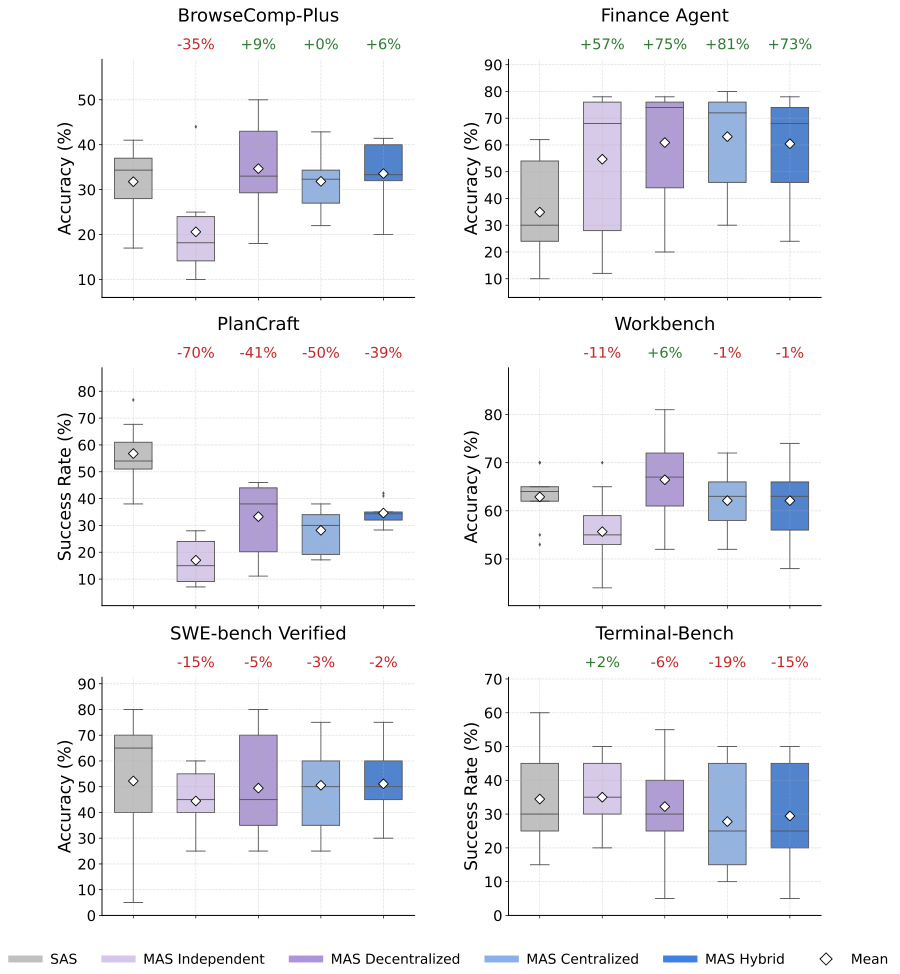
\includegraphics[width=\linewidth,height=0.74\textheight,keepaspectratio]{images/agentic-models-memory/kim_scaling_fig2_boxplots.png}
        \column{0.48\textwidth}
        \begin{itemize}\itemsep0.4em
            \item \textbf{Parallel, read-heavy work wins.} Finance-Agent gains 80.8\% with a centralised team.
            \item \textbf{Sequential, stateful work loses.} Every multi-agent variant degrades PlanCraft, by 39 to 70\%.
            \item \textbf{Coding is neutral or worse.} SWE-bench Verified: $-2.1\%$ at best.
            \item \textbf{Read against write:} research parallelises. Code does not, because actions carry \emph{implicit decisions} that conflict.
        \end{itemize}
    \end{columns}
    \src{Figure: Kim et al., \href{https://arxiv.org/abs/2512.08296}{arXiv:2512.08296}, Figure 2. Yan, ``Don't Build Multi-Agents'' (Cognition, Jun 2025). Chase, ``How and when to build multi-agent systems'' (LangChain, Jun 2025).}
\end{frame}

\begin{frame}{Failure Modes: The MAST Taxonomy}
    \begin{columns}[T,onlytextwidth]
        \column{0.6\textwidth}
        \centering
        \small
        \renewcommand{\arraystretch}{1.15}
        \begin{adjustbox}{max width=\linewidth}\begin{tabular}{>{\raggedright\arraybackslash}p{2.6cm}>{\raggedright\arraybackslash}p{4.1cm}r}
            \toprule
            \textbf{Category} & \textbf{Most frequent modes} & \textbf{Share} \\
            \midrule
            System design & step repetition & 15.7\% \\
            & unaware of termination conditions & 12.4\% \\
            \midrule
            Inter-agent misalignment & reasoning and action mismatch & 13.2\% \\
            & task derailment & 7.4\% \\
            \midrule
            Task verification & incorrect verification & 9.1\% \\
            & no or incomplete verification & 8.2\% \\
            \bottomrule
        \end{tabular}\end{adjustbox}
        \column{0.38\textwidth}
        \begin{itemize}\itemsep0.45em
            \item Built from 150+ traces with six experts. Agreement $\kappa = 0.88$.
            \item \textbf{Failure rates} across seven systems: from 41\% (MetaGPT) to 86.7\% (HyperAgent).
        \end{itemize}
    \end{columns}
    \vspace{0.4em}
    \takeaway{These are \textbf{specification, hand-over and verification} failures: organisational problems, on simple tasks.}
    \src{Cemri et al., ``Why Do Multi-Agent LLM Systems Fail?'' \href{https://arxiv.org/abs/2503.13657}{arXiv:2503.13657} (v3). 14 modes in total. The two most frequent per category are shown.}
\end{frame}

\begin{frame}{Finding the Culprit, and Fixing It}
    \begin{columns}[T,onlytextwidth]
        \column{0.46\textwidth}
        \centering
        \begin{adjustbox}{max width=\linewidth}\begin{tikzpicture}
            \begin{axis}[
                ybar, bar width=14pt, width=6.6cm, height=4.6cm,
                ymin=0, ymax=65, ylabel={attribution accuracy (\%)},
                symbolic x coords={Which agent,Which step},
                xtick=data, x tick label style={font=\scriptsize},
                y label style={font=\scriptsize}, y tick label style={font=\scriptsize},
                nodes near coords, nodes near coords style={font=\scriptsize},
                axis lines*=left, ymajorgrids, grid style={gray!20}, enlarge x limits=0.6]
                \addplot[fill=KAred!45, draw=KAred!75!black] coordinates {(Which agent,53.5) (Which step,14.2)};
            \end{axis}
        \end{tikzpicture}\end{adjustbox}

        {\scriptsize Best automated failure attribution on logs from 127 multi-agent systems (Who\&When).}
        \column{0.52\textwidth}
        \begin{itemize}\itemsep0.45em
            \item \textbf{Debugging is unsolved.} The best method finds the responsible agent half the time, and the decisive step rarely.
            \item \textbf{Tactical fixes help modestly.} A final consensus step: +9.4\%. High-level objective verification: +15.6\%.
            \item \textbf{Structural fixes help more.} Explicit task boundaries for sub-agents, one agent for final synthesis, a central verifier.
        \end{itemize}
    \end{columns}
    \vspace{0.3em}
    \takeaway{\textbf{A fair evaluation} compares at matched token budgets against one agent with self-consistency.}
    \src{Zhang et al., ``Which Agent Causes Task Failures and When?'' \href{https://arxiv.org/abs/2505.00212}{arXiv:2505.00212}. Cemri et al., \href{https://arxiv.org/abs/2503.13657}{arXiv:2503.13657}, Table 5. Hadfield et al. (Anthropic, 2025).}
\end{frame}

\begin{frame}{Multi-Agent Systems: What to Remember}
    \begin{itemize}\itemsep0.6em
        \item Multi-agent systems \textbf{buy accuracy with tokens}: about 15$\times$ chat, with 58 to 515\% coordination overhead.
        \item Debate and model mixing mostly reduce to \textbf{voting and sampling}. Specialised roles and verifiers are what add value.
        \item They pay off on \textbf{breadth-first, read-only, parallel} tasks where one agent is weak. They hurt sequential and write-heavy work.
        \item \textbf{A2A} connects opaque agents horizontally. \textbf{MCP} connects an agent to tools vertically. Both now sit in one foundation.
        \item Failures are organisational, and attributing them automatically does not yet work.
    \end{itemize}
    \vspace{0.4em}
    \takeaway{\textbf{Next.} So far the agent acts and then sees what happened. Can it predict the outcome first, and can we train it in a simulated world?}
\end{frame}
